%-------------------- Packages --------------------%

\documentclass[11pt,a4paper]{report}
\usepackage[utf8]{inputenc}
\usepackage[french]{babel}
\usepackage[T1]{fontenc}
\usepackage{amsmath} %pour les formules maths
\usepackage{amsfonts}
\usepackage{amssymb}
\usepackage{graphicx} %pour inclure des images
\usepackage{hyperref} %pour les lien URLs
\usepackage[left=2cm,right=2cm,top=3cm,bottom=3cm]{geometry}
\usepackage{pifont} %pour les puces spéciales
\usepackage{listings} %pour écrire du code
\usepackage{xcolor} %pour la mise en couleur
\usepackage{multirow} %pour les tableaux
\usepackage{bclogo} %pour des boîtes texte avec un logo


%-------------------- New Colors --------------------%

%Basic

\definecolor{purple}{rgb}{0.6, 0.2, 0.9}

%Dark
\definecolor{dkgreen}{rgb}{0,.6,0}
\definecolor{dkblue}{rgb}{0,0,.6}
\definecolor{dkyellow}{cmyk}{0,0,.8,.3}
\definecolor{dkred}{rgb}{0.6, 0, 0}


%Light
\definecolor{ltblue}{rgb}{0.67, 0.85, 0.9}
\definecolor{ltred}{rgb}{0.8, 0.32, 0.32}
\definecolor{ltgrey}{rgb}{0.94,0.94,0.94}



%-------------------- Config lstlisting --------------------%

\lstset{
language=php,
basicstyle=\ttfamily\tiny, %
identifierstyle=\color{dkred}, %
keywordstyle=\color{dkblue}, %
stringstyle=\color{dkgreen}, %
commentstyle=\it\color{gray}, %
emph=[1]{php},
emphstyle=[1]\color{black},
emph=[2]{if,and,or,else},
emphstyle=[2]\color{dkyellow},
emph=[3]{imap_open, imap_close, imap_fetch_overview, imap_check, imap_list, imap_mail_move, imap_search, imap_fetchstructure			},
emphstyle=[3]\color{dkblue},
emph=[4]{string, int, double, float, private, public, static, bool, resource, array, object},
emphstyle=[4]\color{purple},
columns=flexible, %
tabsize=2, %
extendedchars=true, %
showspaces=false, %
showstringspaces=false, %
numbers=left, %
numberstyle=\tiny, %
breaklines=true, %
breakautoindent=true, %
captionpos=b, %
backgroundcolor=\color{ltgrey}
}

%-------------------------------------%
\newcommand{\vf}[3]{\textcolor{dkblue}{\textit{#1}}\hspace*{.2cm}#2\vspace*{.2cm}\par\hspace*{.5cm}#3}
\newcommand{\qouv}[2]{\textcolor{dkblue}{\textit{#1}}\vspace*{.2cm}\par\hspace*{.5cm}#2}

\newcommand{\vrai}[0]{\textcolor{dkgreen}{Vrai}}
\newcommand{\faux}[0]{\textcolor{dkred}{Faux}}


\author{Wéry Benoît}
\title{Préparation à l'examen de \textit{NoSQL}}
\date{\today}


\begin{document}
\maketitle

%---------------------%
\chapter{Vrai ou Faux}
%---------------------%


\begin{enumerate}\setlength\itemsep{1em}
%--- 1 -------------------------------%
\item\vf{Dans une entreprise, les données vivent souvent plus longtemps que les logiciels.}
{\vrai}
{Une entreprise \textit{utilise} des logiciels et \textit{stocke} des données en veillant à garder le plus d'indépendance possible entre ces deux éléments. Ainsi, un changement d'implémentation de la structure des données ne devrait pas affecter le bon fonctionnement du logiciel.

\paragraph{}
Là où les données doivent persister dans le temps, un logiciel peut être amené à être remplacé (par obsolescance, optimisation,...)
}


%--- 2 -------------------------------%
\item\vf{Dans une entreprise, les logiciels vivent souvent plus longtemps que les données.}
{\faux}
{}


%--- 3 -------------------------------%
\item\vf{Le passage du relationnel au NoSQL se fait généralement au profit d’une diminution des garanties
relatives à la consistence des données.}
{???}
{}


%--- 4 -------------------------------%
\item\vf{Le passage du relationnel au NoSQL se fait généralement au profit d’une diminution de la
quantité de données stockables.}
{\faux}
{... stockables VS stockées...

\paragraph{}
Le NoSQL a émmergé d'un besoin de stocker de nouveaux formats de données (ex: stocker directement des objets plutôt que de devoir retrouver leur informations indépendantes pour le reconstruire), malgré la \textit{puissance} et la \textit{stabilité} des base de données relationnelles, celles-ci ne sont plus suffisantes dans certaines applications.
}


%--- 5 -------------------------------%
\item\vf{Le passage du relationnel au NoSQL se fait généralement au profit de l’abandon de la possibilité
de lire des données de manière concurrente.}
{\faux}
{Le modèle relationnel permet d'accéder de manière concurrente aux données (en R/W) via l'utilisation de \textbf{transactions}, les données sont stockées de façon consistante et persistante.

\paragraph{}
Le modèle NoSQL, quant à lui, permet un accès concurrent aux données MAIS elles ne sont pas garanties consistantes. De plus, les données d'une BDD étant stockées sur des serveurs différents (contrairement au relationnel -> 1machine/BDD), il se peut que des requêtes identiques fournissent des résultats différents. ... A VERIFIER
}


%--- 6 -------------------------------%
\item\vf{Le passage du relationnel au NoSQL se fait généralement au profit d’une diminution des garanties
relatives à la persistance des données.}
{???}
{"la gestion de la persistance des données réfère au mécanisme responsable de la sauvegarde et de la restauration des données. Ces mécanismes font en sorte qu'un programme puisse se terminer sans que ses données et son état d'exécution ne soient perdus". A VERIFIER}


%--- 7 -------------------------------%
\item\vf{Tout comme pour le relationnel, l’organisation des données en NoSQL suit un modèle mathéma-
tique rigoureux.}
{\faux}
{Là où le relationnel se base sur des modèles mathématiques standards pour définir la structure de la BDD, le NoSQL ne suit pas de schéma (ex: possibilité d'ajout de champs sans contrôle). 
\paragraph{}
De cette façon, on obtient une structure \textbf{flexible} avec une BDD qui n'est pas figée dans le temps, ce qui est utile dans le cas de \textit{prototypages}.
}


%--- 8 -------------------------------%
\item\vf{Le NoSQL est particulièrement adapté à des traitements de données de type OLTP}
{\faux}
{\textbf{Rappel: Online Transactional Processing (OLTP)...} modèle qui utilise des données dans un but purement transactionnel -> gestion

\paragraph{}
Une transaction doit faire appel à des données consistantes, ce qui n'est pas garantit dans le cas du NoSQL ... BONNE RAISON?
}


%--- 9 -------------------------------%
\item\vf{Le NoSQL est particulièrement adapté à des traitements de données de type OLAP.}
{\vrai}
{\textbf{Rappel: Online Analytical Processing (OLAP)...} modèle qui utilise les données dans un but d'analyse et de prédictions -> statistiques
}


%--- 10 -------------------------------%
\item\vf{Toutes les bases de données de type NoSQL satisfont les propriétés ACID.}
{\faux}
{\textbf{Rappel: proriétés ACID...}
\begin{itemize}\setlength{\itemsep}{.3em}
\item[$\cdot$]\textbf{A}tomicity: une transaction fait tout ou rien
\item[$\cdot$]\textbf{C}onsistency: la BDD change d'un état valide vers un autre état valide, les données sont constamment à jour
\item[$\cdot$]\textbf{I}solation: une transaction doit être exécutée sans avoir connaissance de l'existance des autres
\item[$\cdot$]\textbf{D}urability: une transcation validée et confirmée est sotckée, durable dans le temps
\end{itemize}

De telles conditions correspondent au modèle relationnel.
\paragraph{}
Un autre ensemble de conditions, le modèle BASE, permet de gérer les \textit{pertes de consistance} en maintenant la fiabilité et correspond donc à l'approche NoSQL:
\begin{itemize}\setlength{\itemsep}{.3em}
\item[$\cdot$]\textbf{B}asically \textbf{A}vailable: le système renverra toujours une réponse, même si la donnée n'est pas à jour ou qu'il s'agit d'un message d'erreur.
\item[$\cdot$]\textbf{S}oft state: l'état change constamment au cours du temps (même lorsqu'il n'y a pas d'inputs) pour essayer de se stabiliser entre les serveurs de la BDD
\item[$\cdot$]\textbf{E}ventual consistency: le système finira tôt ou tard par être consistant
\end{itemize}
}
%--- 11 ----------------------------------------------------------------------------------
\item\vf{Le choix d’architecture peut avoir une influence sur la sécurité du système logiciel.}
{\vrai}
{L'architecture logicielle influence fortement les \textbf{propriétés} du système dont sa sécurité. Par exemple, il est plus difficle d'assurer la sécurité d'un système s'il est distribué (modèle en niveaux) que s'il est sur une unique machine.
\paragraph{}
Comme un choix d'architecture est quasi définitif, il y a des points de \textbf{non retour} lors du développement du système, la phase d'analyse du projet est donc primordiale.
\paragraph{Remarque:} il est \textit{impossible} d'optimiser toutes les propriétés d'un système (performance, sécurité, disponibilité, maintenabilité, fiabilité, tolérance aux pannes, comptabilité,...) car l'amélioration d'un critère se fait bien souvent au détrimant d'un autre. Des choix doivent donc être faits ( = COMPROMIS) quant aux critères les plus pertinents suivant l'application du système.

\paragraph{}
Afin d'améliorer la qualité d'un logiciel, une solution consiste à créer plus de tests unitaires pour couvrir le code au plus possible et effectuer soi-même d'avantage de "\textit{tests à la main}" pour évaluer tous les scénarios possibles d'utilisation. 
\paragraph{}Il est à noter que la \textit{qualité logicielle} est une notion très vague. Il faut se baser sur des critères (ex, norme ISO/CEI 9126: capacité fonctionnelle, fiabilité, facilités d'utilisation, performance, maintenabilité) et définir la façon de les mesurer pour avoir une évaluation qui a du sens.
}


%--- 12 ----------------------------------------------------------------------------------
\item\vf{Un design pattern est un template de code applicable automatiquement étant donné la spécifica-
tion d’une procédure/fonction/méthode.}
{\faux}
{Un design pattern est un \textbf{modèle de conception} général qui répond à une problématique récurrente en développement. Il s'agit d'une desciption de solution dont l'implémentation doit être adpatée aux cas particulier.
\paragraph{}Un pattern n'est donc pas automatiquement applicable.

\paragraph{Remarque:} les patterns sont regroupés selon 3 catégories:
\begin{enumerate}
\item \textbf{construction}: concerne l'instanciation des classes
\item \textbf{structuraux}: concerne l'organisation des classes entre elles
\item \textbf{comportementaux}: concerne la communication entre les objets
\end{enumerate}
}


%--- 13 ----------------------------------------------------------------------------------
\item\vf{Le design pattern du GoF Singleton permet de créer des instances d’une classe une à la fois.}
{\faux}
{Le pattern Singleton a pour objectif de garantir qu'une classe ne puisse être instanciée au plus que une seule fois.
\paragraph{}
Pour ce faire, on rend le constructeur privé (donc accessible uniquement depuis l'intérieur de la classe elle-même) et passe par une méthode pour instancier la classe. Cette méthode garantit qu'il n'existe que une seule instance au plus.
}


%--- 14 ----------------------------------------------------------------------------------
\item\vf{Le design pattern du GoF Builder est de type construction.}
{\vrai}
{L'objectif du pattern Builder est de déléguer la construction d'un objet à une autre classe afin de séparer la construction de l'implémentation.
\paragraph{}Il est utilisé, par exemple, dans le cas d'une classe ayant beaucoup de paramètres dans son constructeur ou plusieurs possibilités d'instanciation avec différentes règles.
\paragraph{}
Pour ce faire, le pattern utilise une classe abstraite qui définit un comportement commun à la création des objets et des classes concrètes, qui étendent celle-ci, pour définir les différents cas possibles de création. Une autre classe, quant à elle, passe par un de ces \textit{builders} concrets pour instancier la classe abstraite.
}


%--- 15 ----------------------------------------------------------------------------------
\item\vf{Pour appliquer le design pattern du GoF Facade, il faut impérativement rendre toutes les
procédures/fonctions/méthodes des sous-systèmes à cacher privées.}
{\faux}
{Le pattern façade est un \textbf{point d'entrée} pour un sous-système, il facilite l'accès à toutes ses fonctionnalités. La façade délègue les requêtes du client aux objets appropriés. Cependant, il s'agit d'une \textit{alternative simplifiée} pour utiliser le système, elle ne bloque pas l'accès individuel aux différentes classes (\textbf{pas d'encapsulation} !)
\paragraph{}
L'intérêt du pattern est de diminuer le couplage entre le client et les classes du sous-système. La façade fait le lien avec les différentes interfaces du sous-système de sorte que l'implémentation des classes ou du client peut changer sans impacter le fonctionnement.
\paragraph{}
Le client peut donc au choix utiliser une des façades du système pour accéder à ses fonctionnalités ou instancier directement une partie du système.
}


%--- 16 ----------------------------------------------------------------------------------
\item\vf{Le design pattern du GoF Template permet d’implémenter un algorithme incomplet avec des
« trous » à remplir (hooks).}
{\vrai}
{Le pattern Template ou Strategy permet de définir une \textbf{famille d'algorithmes} et de choisir dynamiquement (lors de l'exécution) celui à utiliser.
\paragraph{}
Pour cela, le pattern utilise une classe abstraite (la \textit{Stratégie}) qui définit une méthode avec les parties communes d'un algorithme et des trous, représentant les parties variables, qui devront être remplis par des classes concrètes qui étendent cette \textit{Stratégie}. Pour choisir l'algorithme a utiliser, le client possède une variable du type de la classe abstraite et il instancie une des classes conrètes au choix.
}


%--- 17 ----------------------------------------------------------------------------------
\item\vf{La programmation impérative met l’accent sur le comment un programme fonctionne.}
{}
{}


%--- 18 ----------------------------------------------------------------------------------
\item\vf{La programmation déclarative met l’accent sur le comment un programme fonctionne.}
{}
{}


%--- 19 ----------------------------------------------------------------------------------
\item\vf{La programmation fonctionnelle est plus proche de l’impérative que de la déclarative.}
{}
{}


%--- 20 ----------------------------------------------------------------------------------
\item\vf{La programmation fonctionnelle est plus éloignée de l’impérative que de la déclarative.}
{}
{}
%--- 21 -------------------------------%
\item\vf{Dans une base de données clé-valeur, il est généralement prévu de rechercher toutes les clés dont
les valeurs satisfont une certaine propriété.}
{\faux}
{La clé étant de type \textit{string}, elle est utilisé pour définir des formats/patterns utilisés pour des recherches efficaces.
\paragraph{COMPLETER[...] slide 27}}


%--- 22 -------------------------------%
\item\vf{Il est possible d’imposer des contraintes sur les domaines des valeurs des paires clé-valeur d’une base de données clé-valeur.}
{}
{COMPLETER [...]}


%--- 23 -------------------------------%
\item\vf{Distribuer les données sur un cluster de machines fait partie des éléments mis en place dans le
monde NoSQL.}
{\vrai}
{Le modèle NoSQL se prête bien à la distribution des données (agrégats) sur différentes machines physiques ( = clusters, architecture en noeuds). 

\paragraph{Intérêts du cluster...} 
\begin{itemize}
\item[$\cdot$] gestion de grandes quantités de données, \textit{scale out}: la capicité de stockage peut être facilement augmentée en ajoutant de nouvelles machines et ce "à chaud" 
\item[$\cdot$] meilleur trafic R/W: la répartition de la charge permet de fluidifier le trafic des requêtes
\item[$\cdot$]résister à des ralentissements, pannes réseaux: les machines peuvent être inscrites chez différents Fournisseurs d'Accès Internet (FAI) et le réseau est de ce fait moins sensible à une éventuelle panne chez un FAI ou une saturation
\end{itemize}
 }


%--- 24 -------------------------------%
\item\vf{Il est possible de faire du sharding de données pour une base de données se trouvant sur une
machine unique.}
{\vrai ? (via machine virtuelle) -> mais complètement inutile}
{Le sharding est une technique de distribution des données qui consiste à répartir la charge entre différents serveurs de façon horizontale ( = [...]).
\paragraph{}
En sharding, les données \textbf{ne sont pas répliquées} et chaque serveur est accessible en \textbf{R/W}. Pour optimiser la distribution, on veillera à rassembler sur un même noeud les données qui sont \textit{accédées ensemble} (probabilité d'accès commun et localisation géographique). C'est le client qui a connaissance de la répartition des données et qui est donc responsable d'interroger la bonne machine.
\begin{figure}[!h]
\center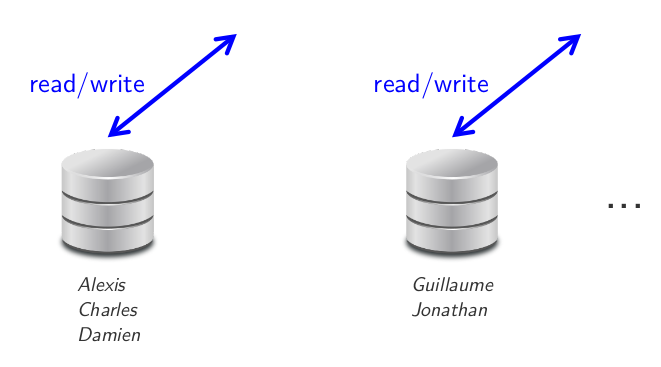
\includegraphics[scale=.3]{images/sharding}
\caption{Distribution des données: modèle sharding \cite{ref1}}
\end{figure}

\paragraph{Avantages:}
\begin{itemize}\setlength{\itemsep}{.2em}
\item[\textcolor{dkgreen}{\ding{52}}]fraction de la DB pour accélérer son traîtement et la rendre plus facile à gérer
\item[\textcolor{dkgreen}{\ding{52}}]avantages cluster (résistance aux pannes, \textit{scale out}, ...)
\end{itemize}

\paragraph{Inconvénients:}
\begin{itemize}\setlength{\itemsep}{.2em}
\item[\textcolor{dkred}{\ding{56}}]définir bonne répartition des données -> risque de surcharge d'un serveur
\item[\textcolor{dkred}{\ding{56}}]pas de résilience (ni en lecture, ni en écriture) -> si un serveur tombe, une partie de la DB n'est plus du tout accessible
\end{itemize}

}


%--- 25 -------------------------------%
\item\vf{Le sharding permet de récupérer les données en cas de corruption grâce à un stockage redondant
de ces dernières sur plusieurs serveurs pouvant être physiquement à des endroits différents.}
{\faux}
{En sharding les données ne sont pas répliquées contrairement aux modèles de réplications \textit{master/slave} ou \textit{peer-to-peer}.}


%--- 26 -------------------------------%
\item\vf{Réplication de données et sharding sont incompatibles.}
{\faux}
{Il est possible de combiner les techniques de \textit{sharding} et \textit{replication} ce qui offre les avantages de résilience (R, W ou les deux) et de répartition de la DB.
\paragraph{}
On peut combiner le sharding avec:
\begin{itemize}
\item[$\cdot$]le \textit{master/slave}: plusieurs maîtres (responsable chacun d'une partie de la DB) ou rôle mixtes (esclave pour certaines données et maîtres pour d'autres)
\item[$\cdot$]le \textit{peer-to-peer}: fraction de la DB (sharding) et réplication sur N noeuds
\end{itemize}
}


%--- 27 -------------------------------%
\item\vf{La réplication master-slave offre la propriété de résilience à la lecture.}
{\vrai}
{Dans le modèle de réplication master/slave, on distingue deux types de noeuds
\begin{enumerate}
\item le \textbf{master}: responsable des données et de leur mise à jour, il est accessible en R/W
\item les \textbf{slaves}: répliques complètes (!!) du maître, accessibles seulement en lecture
\end{enumerate}

\paragraph{}
Les requêtes des clients sont redirigées suivant que ce soit pour de la lecture ou de l'écriture. Comme le master est le seul accessible en lecture, il doit communiquer ses modifications aux esclaves pour les mettre à jour.

\paragraph{}
Ce modèle possède la propriété de \textit{read resilience}, càd que si le maître crash, le système sera toujours accessible en lecture via les esclaves. De plus, il est possible d'élir (manuellement ou automatiquement) un esclave comme nouveau maître si celui-ci tombe.

\begin{figure}[!h]
\center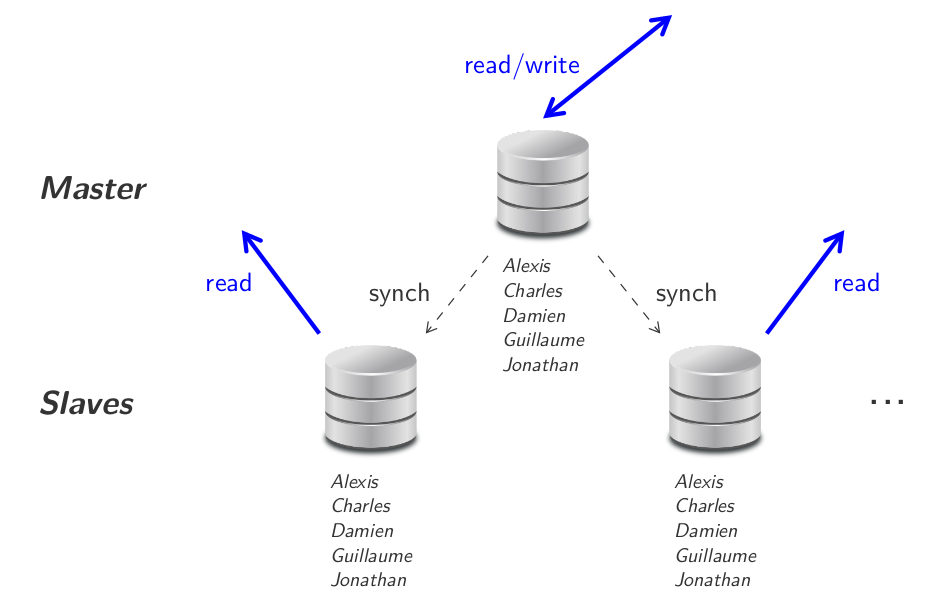
\includegraphics[scale=.3]{images/replication-masterslave}
\caption{Distribution des données: modèle de réplication master/slave \cite{ref1}}
\end{figure}

\paragraph{Avantages:}
\begin{itemize}\setlength{\itemsep}{.2em}
\item[\textcolor{dkgreen}{\ding{52}}]robustesse en cas de crash et \textit{read resilience}
\item[\textcolor{dkgreen}{\ding{52}}]fluidification du trafic pour les requêtes de lecture
\item[\textcolor{dkgreen}{\ding{52}}]avantages cluster (résistance aux pannes, \textit{scale out}, ...)
\end{itemize}

\paragraph{Inconvénients:}
\begin{itemize}\setlength{\itemsep}{.2em}
\item[\textcolor{dkred}{\ding{56}}]pas adapté lorsqu'il y a beaucoup d'écritures -> surcharge maître
\item[\textcolor{dkred}{\ding{56}}]nécessite plus d'espace de stockage puisque chaque noeud est une copie complète du maître
\item[\textcolor{dkred}{\ding{56}}]les valeurs lues par plusieurs utilisateurs peuvent être différentes par inconsistence -> la cohérence des données n'est pas garantie, puiqu'il faut que le maître ait synchronisé ses modifications avec les esclaves
\end{itemize}
}


%--- 28 -------------------------------%
\item\vf{En utilisant une réplication master-slave, les données deviennent complètement inaccessibles une
fois que le master tombe.}
{\faux}
{Par la propriété de \textit{read resilience}, les données seront toujours accessibles en lecture si le maître crash (avec risque de perte d'information si l'esclave n'était pas à jour par rapport au maître). Elles ne seront disponibles en écriture \textbf{que si} un esclave est désigné pour remplacer le maître (-> pas \textit{write resilience})}


%--- 29 -------------------------------%
\item\vf{La consistence des données est plus compliquées à garantir avec une réplication master-slave
qu’avec une réplication peer-to-peer.}
{\vrai}
{Dans le modèle de réplication \textit{peer-to-peer}, les noeuds sont tous égaux, ils sont \textbf{accessibles en lecture et en écriture}. A chaque écriture sur un noeud, tous les autres doivent être mis à jour, ce qui peut créer des conflits d'écriture concurrente si une même donnée est modifiée à deux endroits différents en même temps.
\begin{figure}[!h]
\center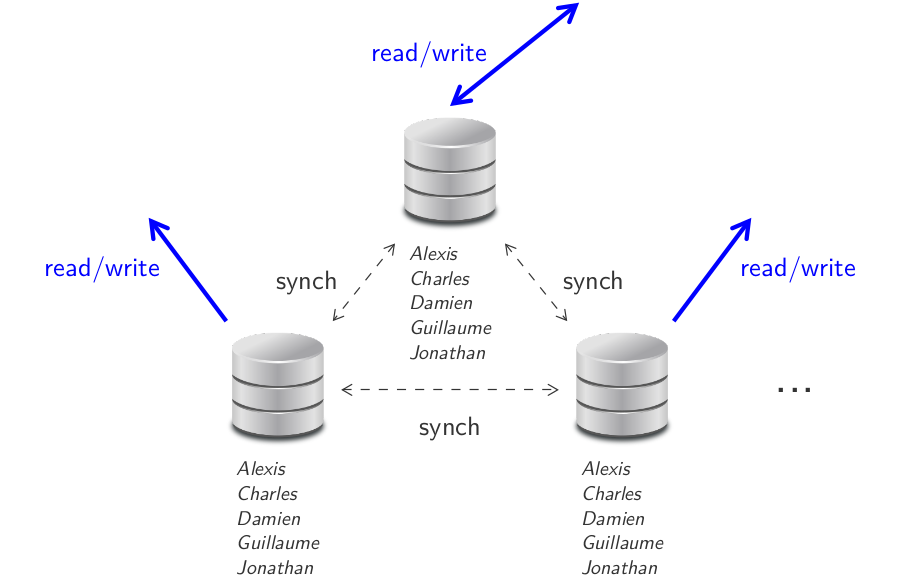
\includegraphics[scale=.3]{images/replication-peertopeer}
\caption{Distribution des données: modèle de réplication peer-to-peer \cite{ref1}}
\end{figure}

\paragraph{Avantages:}
\begin{itemize}\setlength{\itemsep}{.2em}
\item[\textcolor{dkgreen}{\ding{52}}]robustesse en cas de crash et \textit{complete resilience}
\item[\textcolor{dkgreen}{\ding{52}}]fluidification du trafic pour les requêtes de lecture ET d'écriture
\end{itemize}

\paragraph{Inconvénients:}
\begin{itemize}\setlength{\itemsep}{.2em}
\item[\textcolor{dkred}{\ding{56}}]pas adapté lorsqu'il y a beaucoup d'écritures -> lourdeur synchronisations
\item[\textcolor{dkred}{\ding{56}}]nécessite plus d'espace de stockage puisque chaque noeud contient toute la DB
\item[\textcolor{dkred}{\ding{56}}]risques de conflits d'écritures concurrentes
\item[\textcolor{dkred}{\ding{56}}]peu évoluable -> l'ajout d'un nouveau noeud impose de le connecter à TOUS les autres noeuds existants
\end{itemize}
}


%--- 30 -------------------------------%
\item\vf{La consistence des données est plus compliquées à garantir avec une réplication peer-to-peer
qu’avec une réplication master-slave.}
{\faux}
{En master/slave, les modifications peuvent \textbf{seulement} être effectuées via le maître. Il y a donc des risques d'inconsistence des données le temps que les esclaves soient mis à jour MAIS les modifications seront partout les mêmes.
\paragraph{}
En peer-to-peer, des modifications peuvent être faites \textbf{sur n'importe quel noeud} qui communique ensuite à tous les autres ses modifications. Des écritures concurrentes sur différents noeuds peuvent donc engendrer des problèmes d'inconsistence de données qui sont plus difficile à vérifier. (Rem: une solution serait de synchroniser tous les noeuds sur une même date/heure et d'utiliser un serveur dédié pour stocker les informations de mise à jour des données. Ainsi, on peut facilement déterminer la plus récente)
}

%--- 31 -------------------------------%
\item\vf{En utilisant une réplication master-slave, une lecture sur le master assurera toujours d’obtenir
les données les plus récentes}
{}
{}


%--- 32 -------------------------------%
\item\vf{Les buckets de Riak permettent de segmenter les données en plusieurs collections d’agrégats.}
{}
{}


%--- 33 -------------------------------%
\item\vf{On ne peut pas stocker des arbres binaires comme valeurs avec Redis.}
{}
{}


%--- 34 -------------------------------%
\item\vf{Redis garantit la persistance de données.}
{}
{}


%--- 35 -------------------------------%
\item\vf{Les bases de données orientée colonnes optimisent le stockage disque pour des tables qui
contiennent de nombreuses lignes.}
{}
{}


%--- 36 -------------------------------%
\item\vf{Une base de données orientée colonnes est très adaptée lorsqu’on a plus d’opérations d’écriture
que de lecture.}
{}
{}


%--- 37 -------------------------------%
\item\vf{Une base de données orientée colonnes est très adaptée lorsqu’on a plus d’opérations de lecture
que d’écriture.}
{}
{}


%--- 38 -------------------------------%
\item\vf{Une base de données orientée colonnes est un map à deux niveaux.}
{}
{}


%--- 39 -------------------------------%
\item\vf{Dans une base de données orientée colonnes, les familles de colonnes sont de préférence définies
une fois pour toute lors de la création de la table.}
{}
{}


%--- 40 -------------------------------%
\item\vf{L’avantage de l’utilisation de colonnes plutôt que de lignes est d’offrir une vitesse d’écriture plus grande de nouveaux enregistrements.}
{}
{}

%--- 41 -------------------------------%
\item\vf{L’avantage de l’utilisation de colonnes plutôt que de lignes est d’offrir un meilleur taux de
compression des données stockées.}
{\vrai}
{
En travaillant en colonnes, on peut notamment optimiser les algorithmes en fonction du types des valeurs de la colonne. (Suite réponse Q35)
}


%--- 42 -------------------------------%
\item\vf{L’avantage de l’utilisation de colonnes plutôt que de lignes est d’offrir de meilleures performances lors de la lecture de tous les enregistrements d’une table.}
{\faux}
{
Le modèle orienté-colonnes offre de meilleures performances à la lecture uniquement lorsqu'on travaille sur certaines colonnes de la table, car on utilise les fichiers relatifs à ces colonnes (et non toute la DB).
\paragraph{}
Dès lors que l'on fait une requête sur l'ensemble des enregistrements, la modèle devient un inconvénient car il nécessite d'ouvrir et de traiter TOUS les fichiers contenant les colonnes, ce qui alourdit davantage la lecture par rapport au modèle relationnel.
}


%--- 43 -------------------------------%
\item\vf{Une base HBase peut servir d’input/output de MapReduce (Hadoop)}
{\vrai}
{
HBase est un SGBD orienté-colonne qui s'exécute par dessus le système de fichiers HDFS ( = [...]). Il permet a une base de servir d'input/output de MapReduce.
\paragraph{}
Les données sont organisées dans des "\textit{tables}" identifiables par un nom. Chaque ligne possède une clé unique pour l'identifier et les colonnes sont regroupées en "\textit{familles}" (identifiables par chaines caract.). Toutes les lignes possèdent les même familles de colonnes mais celles-ci peuvent être remplies ou non.
\paragraph{}
En HBase, les données des cellules sont \textit{versionnées}. Les différentes versions sont identifiées par un \textit{Timestamp}.
\paragraph{}
Ainsi, pour obtenir la donnée d'une cellule, il faut préciser: \textit{Table --> Clé --> Famille Col. --> Colonne --> Timestamp}
\paragraph{}
Les \textbf{familles de colonnes sont stockées dans des HFile séparés}, ce qui facilite la structure de la DB et l'indexation des données. L'avantage de HBase est alors de proposer la distribution et la réplication des données sur un \textit{cluster}.
\begin{figure}[h!]
\center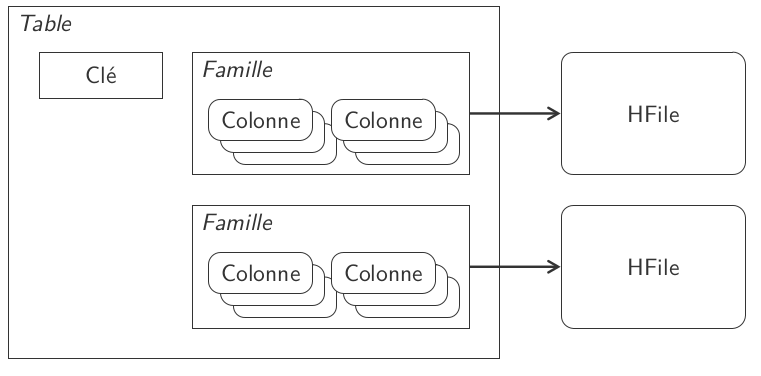
\includegraphics[scale=.3]{images/hbase}
\caption{Modèle de données en HBase \cite{ref1}}
\end{figure}

\paragraph{}
Pour l'écriture des données, celles-ci sont d'abord placées dans un buffer, le \textit{memstore}, qui écrit ensuite les changements dans un HFile [...]
\paragraph{RAPPELS MapReduce...}
}


%--- 44 -------------------------------%
\item\vf{Une base HBase peut servir de fichiers avec GFS (Google File System)}
{???}
{}


%--- 45 -------------------------------%
\item\vf{Une base de données orientée graphe stocke deux collections d’agrégats appelés nœuds et arêtes.}{\vrai}
{Le modèle orienté-graphe stocke deux types d'éléments:
\begin{itemize}
\item[$\cdot$]des \textcolor{ltred}{\textsc{noeuds}}: représentent des entités quelconques avec des propriétés
\item[$\cdot$]des \textcolor{ltred}{\textsc{arêtes}}: représentent des relations UNIDIRECTIONNELLES entre deux noeuds et possèdent une propriété. (\textit{Rem: pour faire un lien bidirictionnel, il faut donc nécessairement utiliser deux arêtes}
\end{itemize}

\paragraph{}
Puisqu'il n'y a pas de restriction sur les types des noeuds/relations, le graphe représente une collection hétérogène d'information dont l'avantage principal est de permettre une \textbf{traversée rapide} des relations, sans que celles-ci ne doivent être reconstruites.

\paragraph{}
Cette architecture est particulière utile dans les cas suivants:
\begin{itemize}
\item[$\cdot$]les collections \textit{très riche de liens} entre les entités
\item[$\cdot$]routage/dispatching et localisation
\item[$\cdot$]moteur de recommandations automatiques
\end{itemize}
}


%--- 46 -------------------------------%
\item\vf{La suppression d’un nœud dans une base de données orientée graphe implique la suppression de
toutes les relations partant et arrivant sur ce nœud.}
{\vrai}
{
Il ne peut \textbf{pas exister de lien mort} dans le graphe, autrement dit la suppression d'un noeud implique nécessairement de supprimer toutes les arêtes adjacentes.
}


%--- 47 -------------------------------%
\item\vf{Il est impossible de stocker une liste de personnes dans une base de données orientée graphe}
{\faux}
{
On distingue différents \textit{types de relations} dans le graphe dont une qui permet de représenter une \textbf{liste chaînée}. La relation est un "pointeur" vers l'élement suivant de la liste.
\begin{figure}[h!]
\center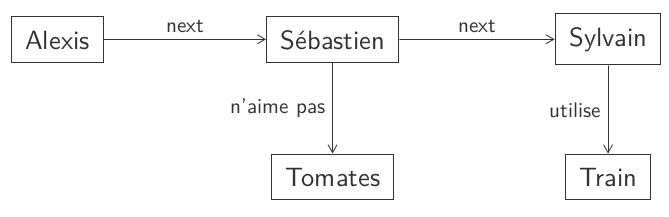
\includegraphics[scale=.3]{images/graphe-relation-liste}
\caption{Représentation d'une liste chaînée en modèle orienté-graphe \cite{ref1}}
\end{figure}
}


%--- 48 -------------------------------%
\item\vf{SPARQL est un langage de requêtes générique permettant d’interroger n’importe quelle base de
données NoSQL.}
{\faux}
{SPARQL (\textit{\textbf{S}PARQL \textbf{P}rotocol and \textbf{R}DF \textbf{Q}uery \textbf{L}anguage)} est un langage de requêtes adapté spécifiquement à la structure des graphes RDF.
\paragraph{}
Tout ceci fait partie de ce qui constitue plus communément le \textbf{Web Sémantique} qui est une extension standardisée du Web, pour l'utilisation de formats de données. Il s'agit donc du \textit{Web des données} qui permet de partager des informations structurées entre des applications. (\textit{« le Web sémantique fournit un modèle qui permet aux données d'être partagées et réutilisées entre plusieurs applications, entreprises et groupes d'utilisateurs »} W3C)
\paragraph{}
Dans ce contexte, le RDF (\textit{\textbf{R}esource \textbf{D}estcription \textbf{F}ormat}) est un \textbf{modèle de graphe} destiné à représenter de façon formelle les ressources web. Il est le langage de base du Web sémantique et permet de stocker les données sous forme de triplets "(Sujet) --- prédicat ---> (Objet)" pour marquer la relation entre deux entités.
\paragraph{}
Le SPARQL, quant à lui, est le langage de requêtes qui interroge les graphes RDF au moyen de quatre types d'instructions:
\begin{enumerate}
\item\textcolor{ltred}{\textsc{select}}: extraire un sous-graphe d'un graphe RD sous forme de table
\item\textcolor{ltred}{\textsc{construct}}: engendrer un nouveau graphe complétant un autre
\item\textcolor{ltred}{\textsc{ask}}: poser une question (True/False)
\item\textcolor{ltred}{\textsc{describe}}: extraire un graphe RDF
\end{enumerate}
}

%--- 49 -------------------------------%
\item\vf{Gremlin est un langage de requêtes générique permettant de décrire des traversées de graphe.}
{\vrai}
{Il est utilisé avec deux types de bases de données:
\begin{itemize}
\item[$\cdot$]OLTP: OrientDB,...
\item[$\cdot$]OLAP: Apache Giraph, Hadoop,...
\end{itemize}
\paragraph{}
Dans ce langage, une requête décrit la traversée à faire pour récupérer des informations, on effectue des opérations sur les noeuds.
}

%--- 50 -------------------------------%
\item\vf{Neo4j supporte les transactions ACID.}
{\vrai}
{Neo4j est un \textbf{système de gestion de graphes} qui supporte les transactions de type ACID et qui interroge les données au moyen du CQL (\textit{\textbf{C}ypher \textbf{Q}uery \textbf{L}anguage}), un langage à travers HTTP (requêtes de types: \textsc{create}, \textsc{match} et \textsc{set}).
\paragraph{}
Il permet d'associer aux noeuds et aux arêtes des \textit{propriétés} sous forme de paires "clé-valeur" et d'ajouter des \textit{labels} aux noeuds, ce qui permet de les regrouper en catégories.
\paragraph{}
Le résultat d'une requête est un \textit{chemin}, càd une séquence de noeuds avec des relations.
}
%--- 51 -------------------------------%
\item\vf{Les bases de données orientée graphe sont très adaptée pour le sharding.}
{}
{}


%--- 52 -------------------------------%
\item\vf{OrientDB offre la possibilité d’utiliser le sharding de données.}
{}
{}


%--- 53 -------------------------------%
\item\vf{Une approche pessimiste de la consistence des données consiste à se limiter à un serveur unique
pour le stockage des données.}
{}
{}


%--- 54 -------------------------------%
\item\vf{Garantir la consistence de lecture empêchera tout conflit de type write-write.}
{}
{}


%--- 55 -------------------------------%
\item\vf{Garantir la consistence de mise à jour empêchera tout conflit de type read-write.}
{}
{}


%--- 56 -------------------------------%
\item\vf{Garantir la consistence de réplication est impossible avec un système peer-to-peer.}
{}
{}


%--- 57 -------------------------------%
\item\vf{Si mes données sont répliquées sur quatre nœuds, avec W = 2, il suffit de lire deux nœuds pour
lire l’information la plus à jour.}
{}
{}


%--- 58 -------------------------------%
\item\vf{Si mes données sont répliquées sur quatre nœuds, il suffit d’impliquer W = 2 nœuds dans
l’écriture pour assurer une consistence des données.}
{}
{}


%--- 59 -------------------------------%
\item\vf{L’utilisation d’un timestamp comme version stamp est moins lourd à déployer que d’utiliser un
GUID (Globally Unique Identifier).}
{}
{}


%--- 60 -------------------------------%
\item\vf{L’utilisation d’un GUID (Globally Unique Identifier) comme version stamp est moins lourd à
déployer que d’utiliser un timestamp.}
{}
{}


%--- 61 -------------------------------%
\item\vf{L’utilisation d’un GUID (Globally Unique Identifier) comme version stamp permet de retrouver
la version la plus récente d’une donnée.}
{}
{}


%--- 62 -------------------------------%
\item\vf{Le write optimiste est très cher à implémenter dans un modèle clé-valeur.}
{}
{}


%--- 63 -------------------------------%
\item\vf{Dans une base de données orientée colonnes, les données transitent par plusieurs espaces de
stockage avant leur destination finale permanent.}
{}
{}


%--- 64 -------------------------------%
\item\vf{Il est possible d’utiliser de la réplication master-slave avec une base de données orientée graphe pour rendre les lectures plus performantes.}
{}
{}


%--- 65 -------------------------------%
\item\vf{Les bases de données orientée documents permettent d’effectuer des transactions atomiques au
niveau d’un document.}
{}
{}


%--- 66 -------------------------------%
\item\vf{Les bases de données orientée documents permettent d’effectuer des transactions atomiques au
niveau d’une collection.}
{}
{}


%--- 67 -------------------------------%
\item\vf{On peut changer le modèle d’une base de données NoSQL entre clés-valeurs, colonnes et
documents, tout en garantissant exactement le même ensemble de propriétés.}
{}
{}


%--- 68 -------------------------------%
\item\vf{Le passage vers le NoSQL permet de se passer des ORMs.}
{}
{}


%--- 69 -------------------------------%
\item\vf{Le NoSQL est très adapté pour stocker des données très uniformes.}
{}
{}

%--- 70 -------------------------------%
\item\vf{Le passage du relationnel au NoSQL rend les calculs à effectuer sur les données plus lents suite à un éventuel cout de transfert des données au sein du cluster.}
{}
{}

%--- 71 -------------------------------%
\item\vf{L’opération Map s’applique à une collection de documents et renvoie un collection modifiée.}
{}
{}


%--- 72 -------------------------------%
\item\vf{L’opération Reduce produit un résultat unique.}
{}
{}


%--- 73 -------------------------------%
\item\vf{ElasticSearch est une base de données NoSQL.}
{}
{}


%--- 74 -------------------------------%
\item\vf{ElasticSearch possède des caractéristiques similaires aux bases de données NoSQL.}
{}
{}


%--- 75 -------------------------------%
\item\vf{Une migration de données en relationnel ou en NoSQL implique toujours un stockage physique
de données redondantes.}
{}
{}

\end{enumerate}

\end{document}
